\section{Overview of Gas-Phase Species Transport}
\label{sec:transport:overview}

%% \subsection{Equal Effective Diffusivities}
%% \label{sec:transport:overview:le1}

%% Summary of equal effective diffusivities approach.


\subsection{Considerations for PAH}
\label{sec:transport:overview:pah}

The nonpremixed flamelet equations for species and temperature were derived in \cref{sec:lesmodels:combust:flamelet} while assuming that species mass fraction and temperature gradients parallel to the mixture fraction gradient dominate and that the species' effective Lewis numbers are unity. The theory behind the latter assumption states that, at sufficiently large Reynolds number, the smallest scales of turbulence (Kolmogorov scales) penetrate the fuel-oxidizer mixing zone of the nonpremixed flame~\cite{peters1984}. Consequently, turbulent mixing dominates molecular mixing within this region, and all species are transported with unity effective Lewis numbers. This line of reasoning implicitly assumes that the species' length scales are comparable to the fuel-oxidizer mixing length scale, which is certainly true for the major combustion products such as \ce{CO}, \ce{CO2}, \ce{H2}, and \ce{H2O}.

However, the DNS studies of Bisetti \etal~\cite{bisetti2012} and Attili \etal~\cite{attili2014} suggest otherwise for PAH, which play an integral role in soot nucleation and condensation. In \cref{fig:transport:overview:pah:unsteadypah}, the mass fractions of acetylene and naphthalene from the DNS are compared to the values from the one-dimensional steady flamelet equation solutions under the same set of conditions (unity Lewis number, no Soret and Dufour effects, same reduced chemical mechanism, etc.). It is evident that, as the scalar dissipation rate is increased, the mass fraction of acetylene falls from $2 \times 10^{-2}$ to $1 \times 10^{-2}$ while the mass fraction of naphthalene decreases two orders of magnitude from $10^{-4}$ to $10^{-6}$. Naphthalene is clearly more sensitive to the local value of scalar dissipation rate, which is a result of its slow formation chemistry. An elevated local scalar dissipation rate minimizes the time for larger hydrocarbon species to collide and successfully react, so the presence of PAH is restricted to a limited range of low scalar dissipation rates.

\begin{figure}[ht]
  \centering
  \begin{subfigure}[b]{0.375\linewidth}
    \centering
    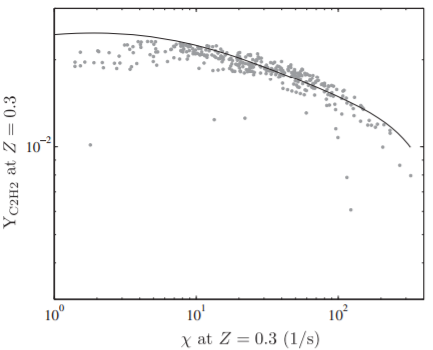
\includegraphics[width=\linewidth]{ch-transport/figures/dns-YC2H2vschi}
  \end{subfigure}%%
  \begin{subfigure}[b]{0.375\linewidth}
    \centering
    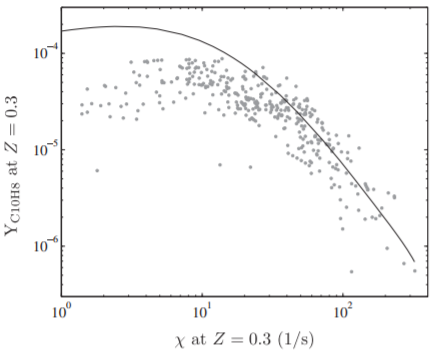
\includegraphics[width=\linewidth]{ch-transport/figures/dns-YC10H8vschi}
  \end{subfigure}
  \caption[Effects of Scalar Dissipation Rate on $Y_{\ce{C2H2}}$ and $Y_{\ce{C10H8}}$]{Mass fraction of acetylene and naphthalene as a function of scalar dissipation rate, reproduced from Bisetti \etal~\cite{bisetti2012}. Samples are taken at $t = 5$ ms and $Z = 0.3$ from the same DNS conditions of \cref{fig:subfilter:zussp:chisensitivity}. Solid lines are the steady flamelet solutions.}
  \label{fig:transport:overview:pah:unsteadypah}
\end{figure} 

Additionally, the steady flamelet solutions tend to capture the overall decreasing trend of the DNS samples for both acetylene and naphthalene, although significant scatter about the steady solution is present for naphthalene. This deviation is caused by naphthalene's inability to adjust to the rapidly changing turbulent flow field and corresponding scalar dissipation rate as a result of its slow chemistry. PAH larger than naphthalene are anticipated to possess similar characteristics. On the other hand, the chemistry of acetylene is much faster, allowing it to persist in regions of larger scalar dissipation rate.
%The scatter is more significant at lower values of scalar dissipation rate, which is due to unsteady flamelet effects~\cite{turbulentcombustion,bisetti2012}.

As a result of the above phenomena, PAH are confined to spatially intermittent regions of low scalar dissipation rate, which are visible in \cref{fig:subfilter:zussp:chisensitivity} for naphthalene. These regions are on the order of the Kolmogorov scale or smaller~\cite{vaishnavi2008}, where transport is solely dictated by molecular diffusion. Therefore, it is worthwhile to examine the effects of molecular transport on the evolution of these soot precursors. Flamelet models that incorporate differential diffusion are presented in the following subsection.


\subsection{Molecular Transport}
\label{sec:transport:overview:lei}

Pitsch and Peters~\cite{pitsch1998} previously derived a set of one-dimensional nonpremixed flamelet equations for flat flames accounting for differential diffusion effects. Assuming variable, non-unity species Lewis numbers and a unity mixture fraction Lewis number, the species equation is given by
\begin{equation}\label{eq:transport:overview:lei:flamelety}
  \rho\pder[Y_k]{\tau} = \frac{\rho\chi}{2 Le_k}\sder[Y_k]{Z} + \dot{m}_k + \frac{\rho\chi}{2 Le_k}\frac{Y_k}{W}\sder[W]{Z} + V_k^{DD},
\end{equation}
where the species Lewis numbers $Le_k = \lambda/c_p\rho D_k$ represent the ratio of thermal to mass diffusivities and $V_k^{DD}$ represents the molecular transport correction terms as outlined in Pitsch and Peters~\cite{pitsch1998}. Similarly, the one-dimensional, adiabatic temperature equation is given by
%, $D_k = (1 - Y_k)/\sum\limits_{k \neq l} (X_k/D_{k,l})$ is the mixture-averaged diffusivity for species $k$, and $\chi = 2D_Z(\partial Z/\partial x_j)^2$ is the scalar dissipation rate. The diffusion velocities are expressed by the Curtiss-Hirschfelder approximation~\cite{curtiss1949} with a velocity correction to enforce mass conservation. These remaining molecular transport correction terms are lumped into $V_k^{DD}$ and are outlined in Pitsch and Peters~\cite{pitsch1998}.
\begin{equation}\label{eq:transport:overview:lei:flamelett}
  \rho c_p \pder[T]{\tau} = \frac{\rho c_p \chi}{2}\sder[T]{Z} + \frac{\rho\chi}{2}\pder[c_p]{Z}\pder[T]{Z} - \sum\limits_{k} h_k\dot{m}_k + \sum\limits_{k} \frac{\rho\chi}{2 Le_k}\left( \pder[Y_k]{Z} + \frac{Y_k}{W}\pder[W]{Z} \right)(c_p - c_{p,k})\pder[T]{Z},
\end{equation}
where $W$ is the molecular weight of the mixture and pressure variations have been neglected. Note that \cref{eq:transport:overview:lei:flamelety,eq:transport:overview:lei:flamelett} have been derived while assuming that the nonpremixed flame is one-dimensional in physical space \textit{a priori}. This assumption is convenient in the limit of a thin, one-dimensional flat flame but is not appropriate for thick or curved flames. Recently, Xuan \etal~\cite{xuan2014} re-derived the flamelet equations accounting for differential diffusion while assuming that the nonpremixed flame is one-dimensional in mixture fraction space \textit{a posteriori} in order to capture curvature effects. Although the latter formulation will not be used in the remainder of this work, curvature effects can significantly affect transport in mixture fraction space. Multidimensional effects were found to improve predictions of soot yield in laminar premixed flames~\cite{xuan2016}, and analysis of curvature effects on PAH evolution in turbulent nonpremixed combustion is a suggestion for future work.

%Although the latter formulation will not be used in the remainder of this work, curvature effects can significantly affect transport in mixture fraction space, and analysis of curvature effects on PAH evolution in turbulent nonpremixed combustion is a suggestion for future work.

Attili \etal~\cite{attili2016} conducted two three-dimensional DNS of the same configuration as previously described in \cref{sec:subfilter:dns}, with a domain size of $L_x \times L_y \times L_z = 105 \times 94 \times 47$ mm. A mixture-averaged transport approach was employed in one DNS, while the other modeled transport of gas-phase species with unity Lewis numbers. These two simulations were compared to analyze the influence of the diffusion model on the flame structure and soot formation. Their results at $t = 15$ ms, shown in \cref{fig:transport:overview:lei:a2vsz}, indicate that acetylene is unaffected by differential diffusion while naphthalene is strongly affected by the molecular transport model. The locations of the peaks for the latter species are the same for both transport models, but the magnitudes vary by more than a factor of two. These trends are consistent across all times in the DNS and suggest the importance of differential diffusion in predicting the yield of naphthalene and other larger PAH. Attili \etal~\cite{attili2016} noted that the mixture-averaged approach lead to smaller amounts of diffusion (larger Lewis number) of naphthalene than the equal diffusivities approach. As a consequence, the naphthalene structures were found to be smaller and characterized by larger peaks. These ultimately affect the formation of soot due to the non-linearity of the soot source terms with respect to the concentration of PAH species.

\begin{figure}[htb]
  \centering
  \includegraphics[width=0.6\linewidth]{ch-transport/figures/DNSComparison-A2-C2H2}
  \caption[DNS Results with $Le = 1$ and $Le \neq 1$, $\langle Y_{\ce{C2H2}}|Z \rangle$ \& $\langle Y_{\text{A2}}|Z \rangle$ vs. $Z$]{Means of acetylene (\ce{C2H2}) and naphthalene (\ce{A2}) mass fraction conditioned on mixture fraction at $t = 15$ ms, reproduced from Attili \etal~\cite{attili2016}. The filled squares are transport with mixture-averaged diffusion, and the open circles are the $Le = 1$ case. The vertical black dashed line marks the location of stoichiometric mixture fraction $Z_{st} = 0.147$.}
  \label{fig:transport:overview:lei:a2vsz}
\end{figure}

On the other hand, it was also observed that the detailed transport model had a less significant influence on predictions of the temperature and the mass fractions of species that participate in the heat-releasing chemistry. In \cref{fig:transport:overview:lei:tvsz}, there is very little difference between the profiles from the two simulations for the temperature and hydroxyl mass fraction. The discrepancy between the transport models is larger for the hydrogen radical mass fraction profile (not shown), although this may be the result of an only moderate Reynolds number. Flamelet solutions with equal effective diffusivities track the unity Lewis number profiles from the DNS fairly well, unlike the solutions with detailed transport, which deviate from the DNS with the corresponding model.

It is clear that there is a simultaneous presence of transport by molecular diffusion for species that are confined to regions on the order of the Kolmogorov scale or smaller and transport by turbulent eddies for species that participate in faster chemistry. A model for gas-phase species transport that attempts to account for unity and non-unity Lewis numbers is presented in the upcoming subsection.

\begin{figure}[htb]
  \centering
  \includegraphics[width=\linewidth]{ch-transport/figures/DNSComparison-T-OH}
  \caption[DNS Results with $Le = 1$ and $Le \neq 1$, $\langle T|Z \rangle$, and $\langle Y_{\ce{OH}}|Z \rangle$ vs. $Z$]{Means of temperature and hydroxyl mass fraction conditioned on mixture fraction at $t = 15$ ms, reproduced from Attili \etal~\cite{attili2016}. The filled squares are transport with mixture-averaged diffusion, and the open circles are the $Le = 1$ case. One-dimensional nonpremixed flamelet solutions are indicated by the dashed lines (mixture-averaged) and solid lines ($Le = 1$). The vertical black dashed line is the same as in \cref{fig:transport:overview:lei:a2vsz}.}
  \label{fig:transport:overview:lei:tvsz}
\end{figure}


\subsection{Bimodal Transport}
\label{sec:transport:overview:bimodal}

% \Cref{eq:transport:overview:lei:flamelety,eq:transport:overview:lei:flamelett} have been observed to overpredict the amount of differential diffusion in the downstream region of a turbulent jet flame~\cite{pitsch2000}. This behavior has been explained by the decreased Reynolds number in that region, where a diminished scalar dissipation rate permits the smallest scales of turbulence to enter the broadened mixing zone.
The flamelet equations of \cref{sec:lesmodels:combust:flamelet} were derived for very high Reynolds number flows, where it is assumed that only turbulent transport is important. Conversely, \cref{eq:transport:overview:lei:flamelety,eq:transport:overview:lei:flamelett} were derived while assuming that only molecular transport matters, which is applicable to laminar flows. However, for a finite Reynolds number, the truth is in between. Recently, Wang~\cite{wang2016} introduced a Reynolds number dependence into the flamelet framework in order to address this point. To measure the degree of differential molecular diffusion, Wang defined a parameter
\begin{equation}\label{eq:transport:overview:bimodal:theta}
  \theta(r)= \frac{r}{1 + r},
\end{equation}
where $r$ is the ratio of the molecular diffusivity to the turbulent diffusivity and is inversely proportional to the Reynolds number. At the limit of an infinite Reynolds number, the influence of molecular diffusion vanishes as transport by turbulent eddies becomes dominant. In this limit, $r$ and $\theta(r)$ both approach zero. Conversely, when the Reynolds number approaches zero in the laminar limit, the effect of molecular diffusion is maximized, and $r$ tends to infinity. For this situation, $\theta(r)$ approaches unity.

Incorporation into \cref{eq:transport:overview:lei:flamelety,eq:transport:overview:lei:flamelett} is achieved by defining an effective Lewis number for species $k$:
\begin{equation}\label{eq:transport:overview:bimodal:lek}
  \hat{Le}_k = \frac{Le_k}{Le_k + \theta(r) \cdot (1 - Le_k)}.
\end{equation}
The form of this nonlinear dependence on $\theta$ was selected based on the analysis of a turbulent mixing layer~\cite{wang2016}. In the limit of infinite Reynolds number, $\theta = 0$ and $\hat{Le}_k = 1$ to model transport by turbulent diffusion. In the laminar limit, $\theta = 1$ and $\hat{Le}_k = Le_k$ to capture the effects of differential diffusion. %This effective Lewis number is not a physical property anymore, but it allows the aforementioned modes of transport to be modeled by simply replacing all instances of $Le_k$ in \cref{eq:transport:overview:lei:flamelety,eq:transport:overview:lei:flamelett}.

Despite its advancements of the flamelet framework, this model is still inappropriate for sooting flames. Wang's approach implicitly assumes that the length scales of all species are on the order of the thickness of the mixing zone, which varies with respect to the turbulent length scales as a function of Reynolds number. As the Reynolds number varies in a certain region, all species are governed by the mode of transport dictated by \cref{eq:transport:overview:bimodal:theta}. However, from \cref{sec:transport:overview:lei}, it is known that PAH are confined to regions that are on the order of the Kolmogorov scale or smaller due to their slow formation chemistry. At these scales, differential molecular diffusion overwhelms transport by turbulent eddies irrespective of the Reynolds number. Therefore, another model must be formulated to account for these properties of PAH and other species that are governed by slow kinetics. An approach that incorporates the idea of differential differential diffusion is introduced in \cref{sec:transport:ssta}.
